\section{Procesja}

\begin{itemize}
      \item Po odmówieniu \textit{Placeat} \ii~ schodzi na posadzkę: odwraca się
            na stronę Ewangelii i dopiero schodzi na dół, wraz z \cc1 klęka na
            oba kolana i odchodzi do sedilli. Tam zdejmuje ornat i manipularz a
            ubiera białą kapę.
      \item W tym czasie formuje się procesja, która z braku miejsca może zacząć
            się poza prezbiterium \footnote{Gdy wszyscy ministranci ustawią
                  procesję do ciemnicy to na znak \cc3 klękają oprócz \aa\aa~ i
                  \ding{63}} (patrz Rys. \ref{fig:procesja2_czw}).
      \item \oo~ idzie po ombrelino i czeka na rozpoczęcie procesji.
      \item Po przebraniu \ii~ wchodzą \tt1 oraz \tt2 . Następuje zasypanie obu
            kadzielnic.
      \item Następnie \ii~ okadza NS, otrzymuje welon naramienny, wchodzi
            stopniami do ołtarza i zabiera puszkę z NS.
      \item \cc1 i \cc2 pomagają z kapą i welonem i podtrzymują łokcie \ii~ w czasie
            procesji. Całość prowadzi, \cc3, który nadaje tempo i kierunek.
            (patrz Rys. \ref{fig:procesja1_czw})
      \item Tak uformowana procesja udaje się do ciemnicy. (patrz Rys.
            \ref{fig:procesja3_czw})
      \item Do ciemnicy wchodzą: \ii, \tt\tt, \cc1 i \cc2, śpiewacy. (patrz Rys.
            \ref{fig:procesja4_czw})
\end{itemize}

\begin{figure}[h]
      \centering
      \begin{minipage}{0.33\linewidth}
            \centering
            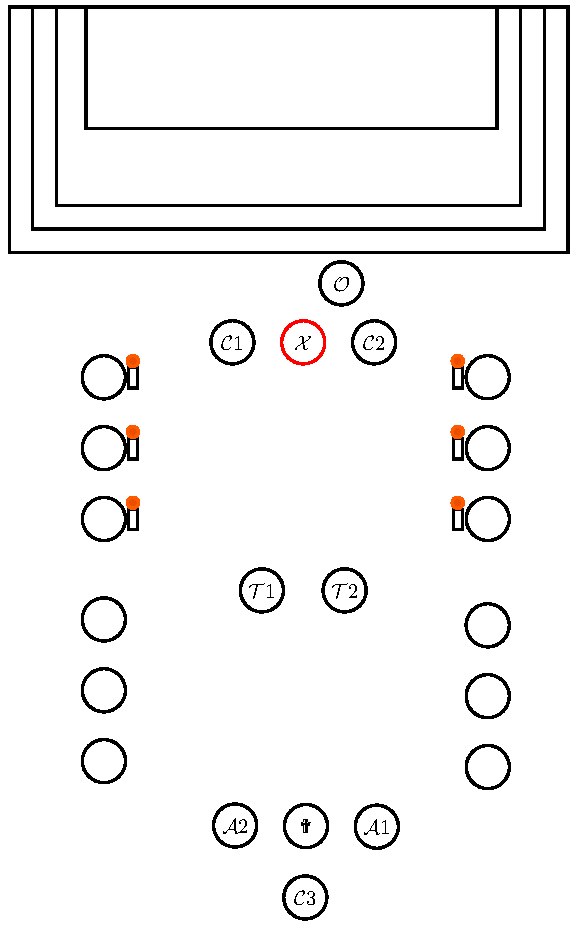
\includegraphics[width=\linewidth]{Figures/Czwartek/Procesja2.pdf}
            \caption{Ustawienie procesji do ciemnicy}
            \label{fig:procesja1_czw}
      \end{minipage}
      \hfill
      \begin{minipage}{0.6\linewidth}
            \centering
            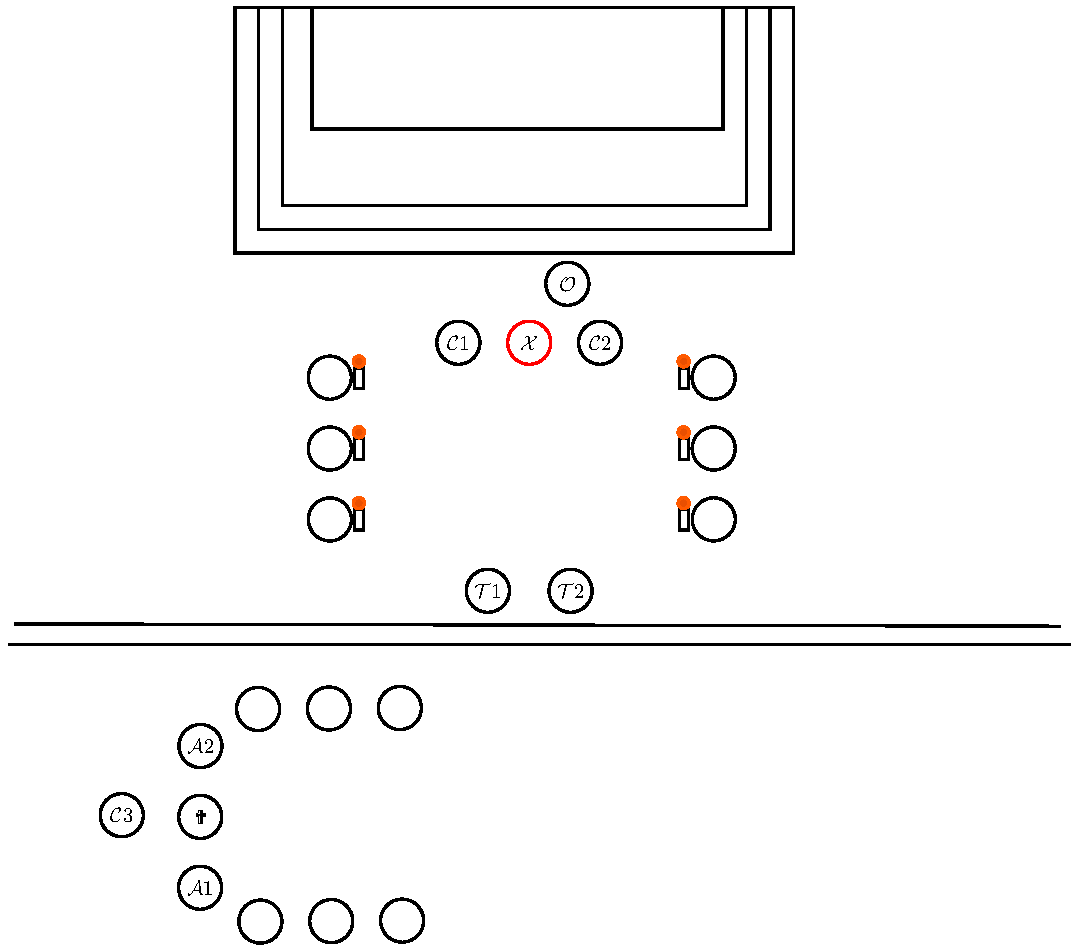
\includegraphics[width=\linewidth]{Figures/Czwartek/Procesja1.pdf}
            \caption{Ustawienie procesji do ciemnicy -- jeśli braknie miejsca}
            \label{fig:procesja2_czw}
      \end{minipage}
\end{figure}
\vfill
\begin{figure}[h]
      \centering
      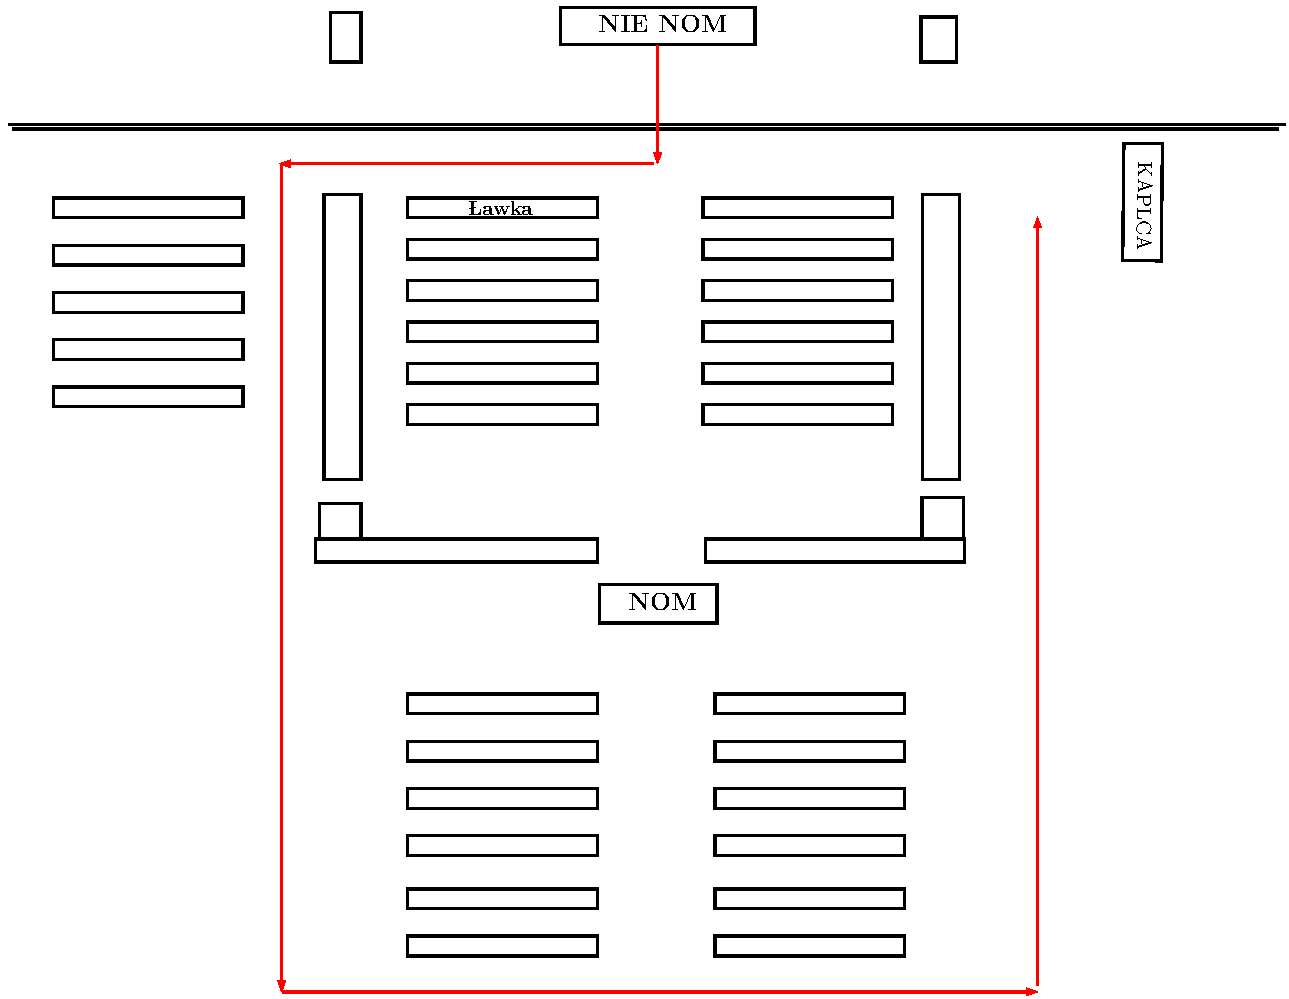
\includegraphics[width=0.7\linewidth]{Figures/Czwartek/Procesja3.pdf}
      \caption{Procesja do ciemnicy}
      \label{fig:procesja3_czw}
\end{figure}
\clearpage
\begin{figure}[h]
      \centering
      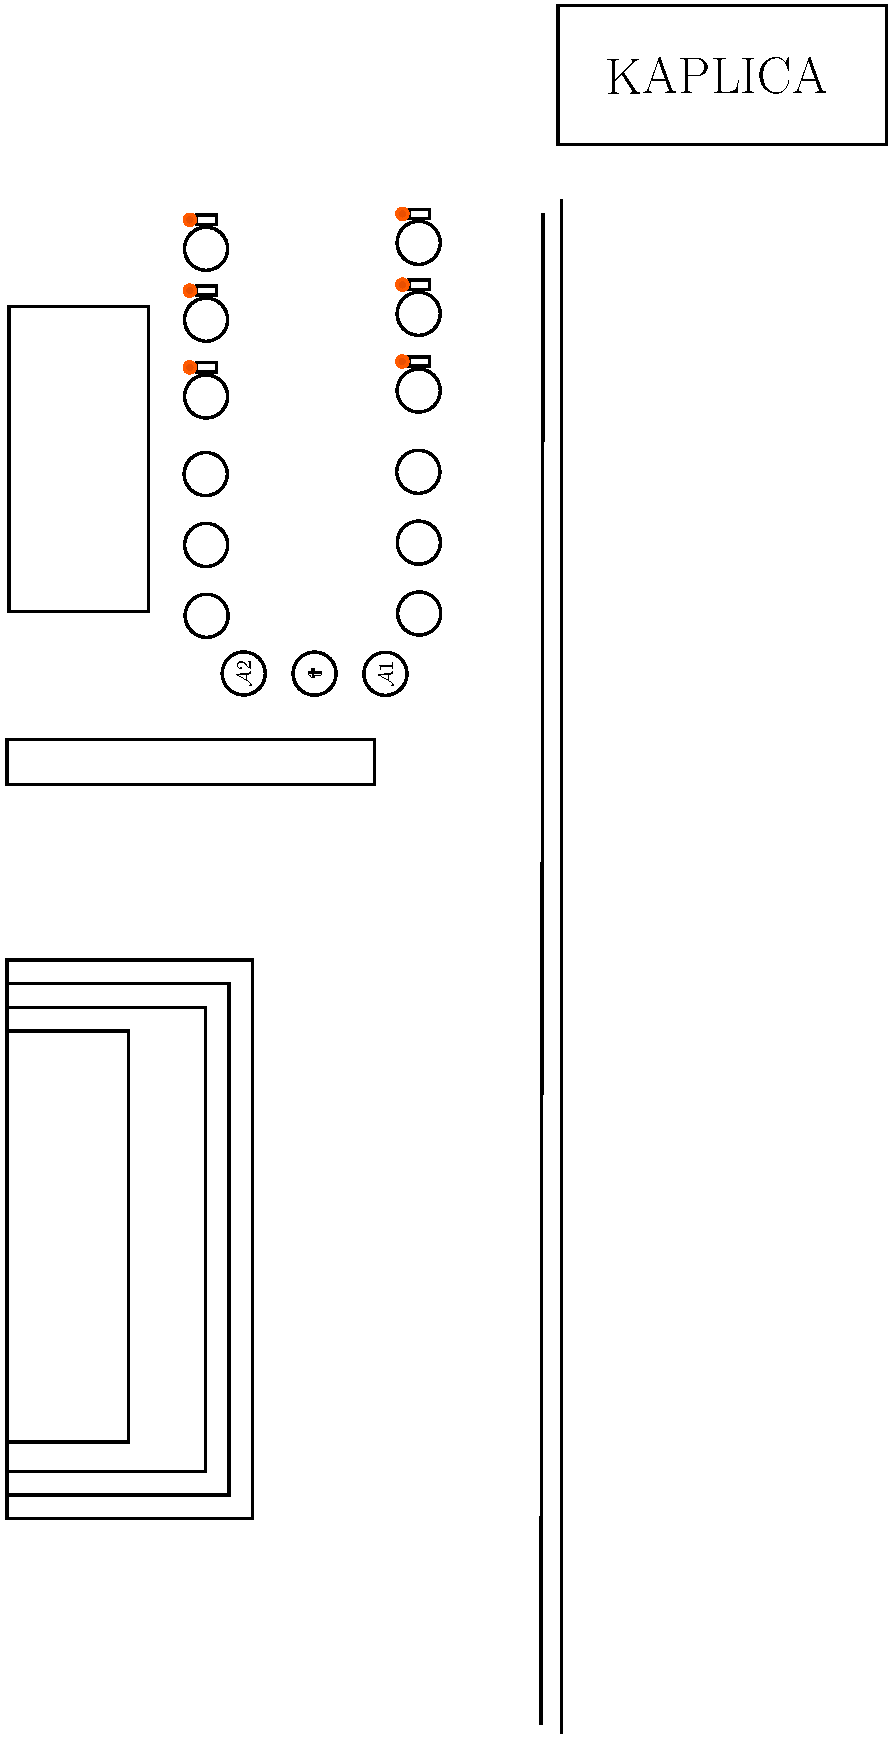
\includegraphics[width=0.5\linewidth,angle=270]{Figures/Czwartek/Procesja4.pdf}
      \caption{Miejsce przeznaczenia ministrantów po dojściu przed kaplicę}
      \label{fig:procesja4_czw}
\end{figure}

\section[W ciemnicy]{W ciemnicy \protect\footnote{Jeśli na ołtarzu zostanie
        dodatkowa puszka to ministranci w składzie: \ii, \cc1 , 2 osoby z
        lucenarium, ministrant z kołatką oraz \oo~ wracają po drugą puszkę do
        ołtarza. Wówczas wszyscy klęczą. Po schowaniu drugiej puszki reszta
        czynności toczy się według instrukcji.}}

\begin{itemize}
      \item Po dojściu do ciemnicy \ii~ stawia puszkę z NS na ołtarzu, przyklęka
            i schodzi na najniższy stopień.
      \item Zaczyna się śpiewać \textit{Tantum ergo} bądź \textit{Przed tak
                  wielkim sakramentem}. W czasie ostatniej zwrotki celebrans
            wstaje i bez błogosławieństwa nakłada kadzidło i okadza NS.
      \item Po skończeniu hymnu wstaje i wstawia NS do tabernakulum. Gdy \ii~
            schowa NS schola zaczyna śpiew ludowy.
      \item Zamieszanie poza kaplicą zimową:
            \begin{itemize}
                  \item \aa~ odstawiają akolitki na kredencje głównego
                        ołtarza i zabierają ze sobą biret \ii. Po wyjściu
                        wiernych dołączają do \ii~ w kaplicy zimowej.
                  \item \ding{63} wstawia krzyż do stojaka.
                  \item Ministranci wyznaczeni do śpiewu psalmu oczekują przed
                        stopniami ołtarza na obnażenie.
                  % \item \cc3 prowadzi 13 ministrantów przed ołtarz MB. Tam stoją
                  %       przed ławkami zwróceni w stronę ołtarza podczas
                  %       obnażania jak i w czasie Ewangelii na Mandatum . Wchodzą
                  %       na stopnie podczas przebierania się \ii do Mandatum.
                  % \item Gdy wszystkie rzeczy do kolejnych celebracji będą
                  %       gotowe \cc2 stopuje śpiew i prosi wiernych o przejście
                  %       do ołtarza MB Zwycięskiej.
                  % \item Reszta ministrantów, którzy wówczas nie będą mieli
                  %       zajęcia idą wraz z wiernymi przed ołtarz MB.
                  \item Do kaplicy zimowej wracają : \cc2, \aa\aa
            \end{itemize}
\end{itemize}
